\chapter[Evaluation]{Evaluation}
\label{cp:evaluation}

{
\parindent0pt
This chapter will present the scenarios and criteria used to evaluate our implementation. Additionally, the results of these benchmarks are reported.
}


\section{Benchmarking Scenarios}
As to not limit our analysis to one specific simulation setting, we use a selection of benchmarking scenarios. These represent different structures as they may be used in real-world applications.
The heating-sphere and exploding-liquid scenarios are identical to the ones given by Newcome et al., the configuration files have been adapted and parametrized for use in this thesis \cite{Newcome2025}.
The other scenarios are are taken from the AutoPas \texttt{md-flexible} example. %TODO: citation


\subsection{Equilibrium}
\label{subsec:equil}
%In the equilibrium scenario, particles with initial velocity $0$ are packed tightly into a cube. Initially, the particles 

% TODO: calculate real time by multiplying iteration with delta t

\begin{figure}[htpb]
	\centering
	\begin{subfigure}[c]{.3\textwidth}
		% \includegraphics[width=\textwidth]{equilibrium/render/t0.png}
		\subcaption{State at $t=0$}
	\end{subfigure}%
	\begin{subfigure}[c]{.3\textwidth}
		% 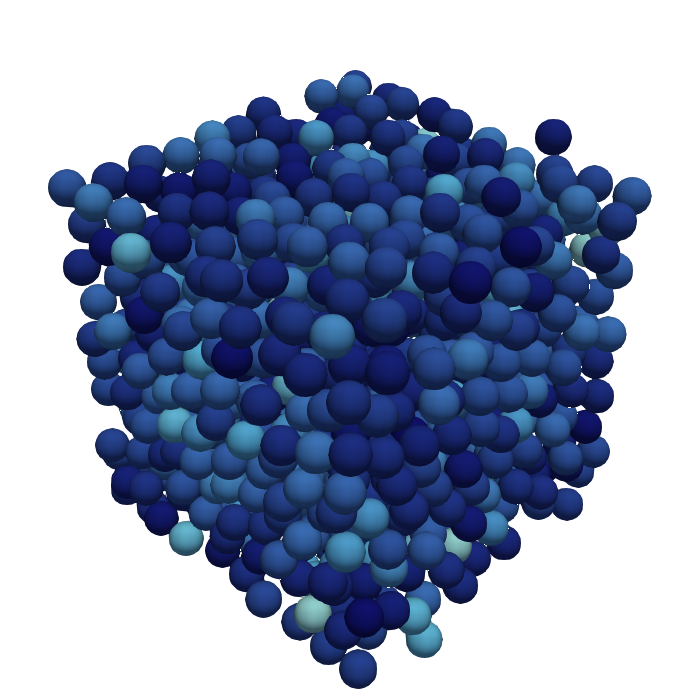
\includegraphics[width=\textwidth]{equilibrium/render/t10000.png}
		\subcaption{State at $t=10000$}
	\end{subfigure}%
	\begin{subfigure}[c]{.3\textwidth}
		% 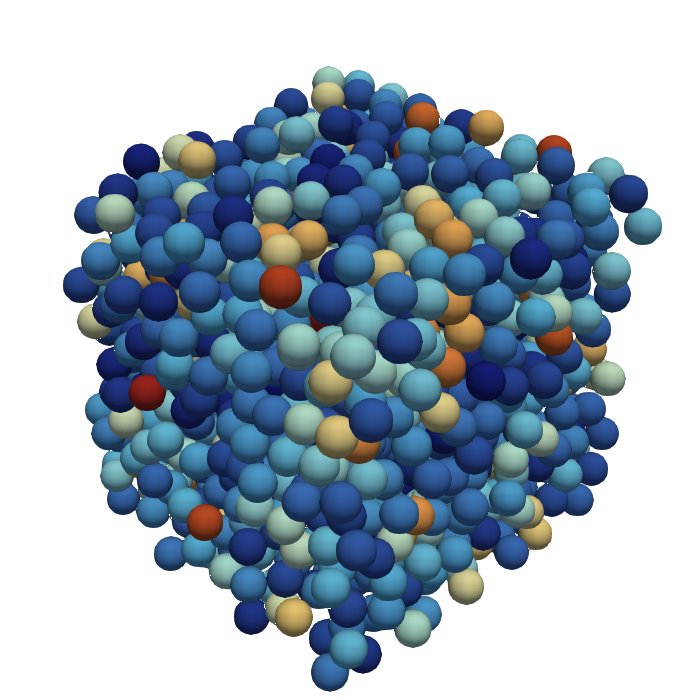
\includegraphics[width=\textwidth]{equilibrium/render/t50000.png}\cite{Newcome2025}
		\subcaption{State at $t=50000$}
	\end{subfigure}%
	\hfill\begin{subfigure}[c]{.08\textwidth}
		\resizebox{\textwidth}{!}{
		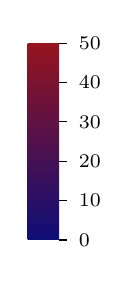
\begin{tikzpicture}
			\def\minval{0}
			\def\maxval{50}
			\definecolor{startcolor}{RGB}{14,14,120}
			\definecolor{midcolor}{RGB}{229,241,196}
			\definecolor{endcolor}{RGB}{150,20,30}
			\def\height{2.5}
			\def\width{0.4}
			\def\nsteps{5}
			
			\shade[top color=endcolor, color=midcolor, bottom color=startcolor] (0,0) rectangle (-\width,\height);
			
			\foreach \i in {0,...,\nsteps}{
			   \pgfmathsetmacro{\val}{\minval + (\maxval-\minval)*\i/\nsteps}
				\pgfmathsetmacro{\y}{\height * (\val-\minval)/(\maxval-\minval)} 
				\draw (0.1,\y) -- (0,\y);
				\node[right, align=left] at (0.125,\y) {\scriptsize\pgfmathprintnumber[fixed,precision=2]{\val}};
			}
			% TODO: add unit for scale
		\end{tikzpicture}
	}
	\end{subfigure}
	\label{fig:evolution_equil}
	\caption{Evolution of the simulation state in the equilibrium scenario.}
\end{figure}


\subsection{Exploding Liquid}
\label{subsec:expl}
\begin{figure}[htpb]
	\centering
	\begin{subfigure}[c]{.3\textwidth}
		% \includegraphics[width=\textwidth]{exploding-liquid/render/t0.png}
		\subcaption{State at $t=0$}
	\end{subfigure}%
	\begin{subfigure}[c]{.3\textwidth}
		% 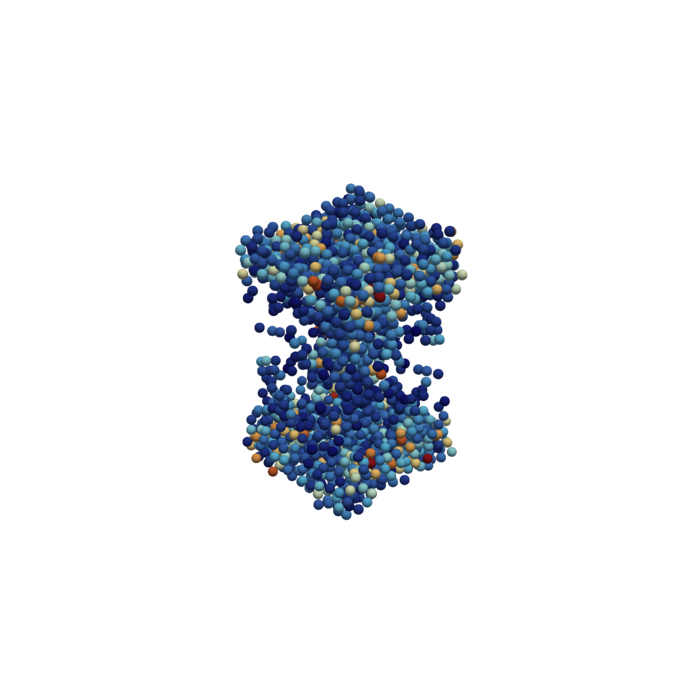
\includegraphics[width=\textwidth]{exploding-liquid/render/t3000.png}
		\subcaption{State at $t=3000$}
	\end{subfigure}%
	\begin{subfigure}[c]{.3\textwidth}
		\centering
		% 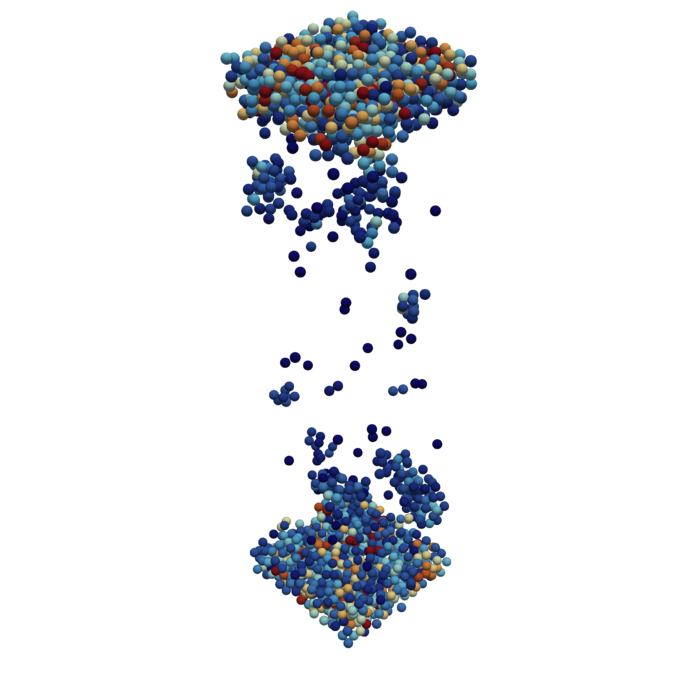
\includegraphics[width=\textwidth]{exploding-liquid/render/t11000.png}
		\subcaption{State at $t=11000$}
	\end{subfigure}
	\hspace*{.15\textwidth}
	\begin{subfigure}[c]{.3\textwidth}
		% 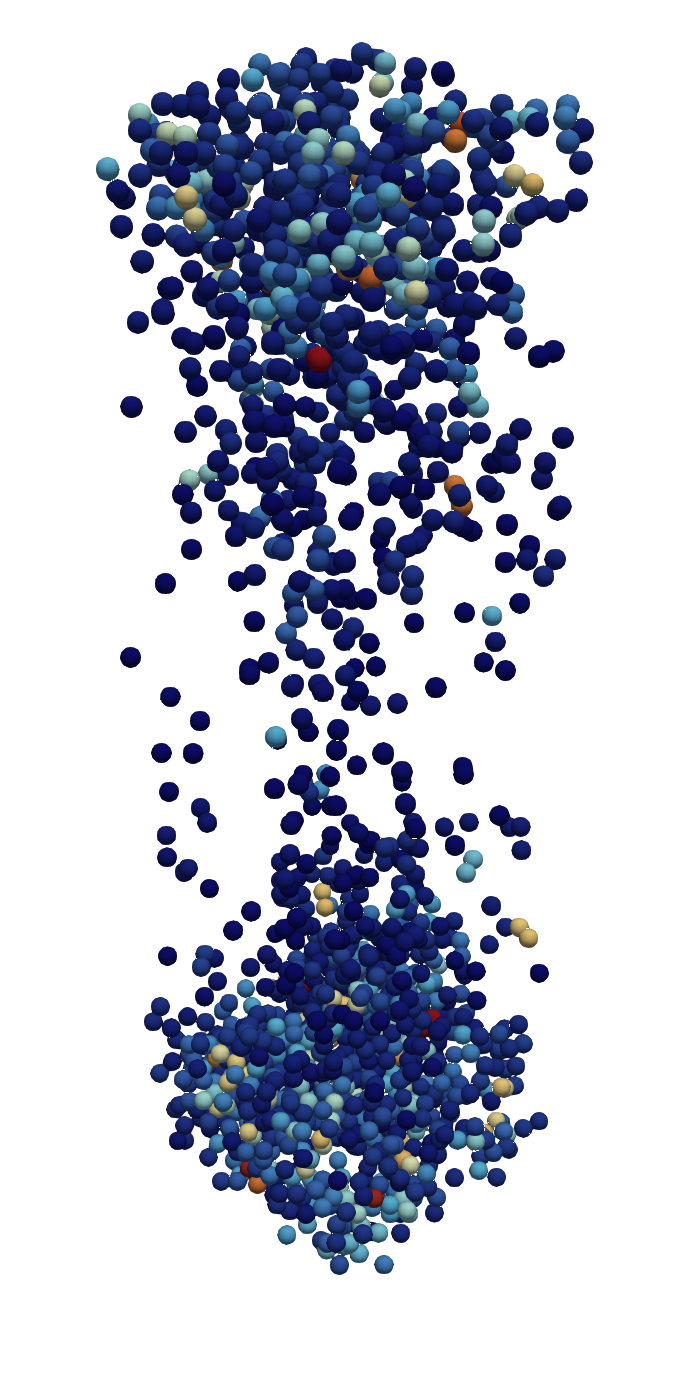
\includegraphics[width=\textwidth]{exploding-liquid/render/t22000.png}
		\subcaption{State at $t=22000$}
	\end{subfigure}%
	\begin{subfigure}[c]{.3\textwidth}
		% 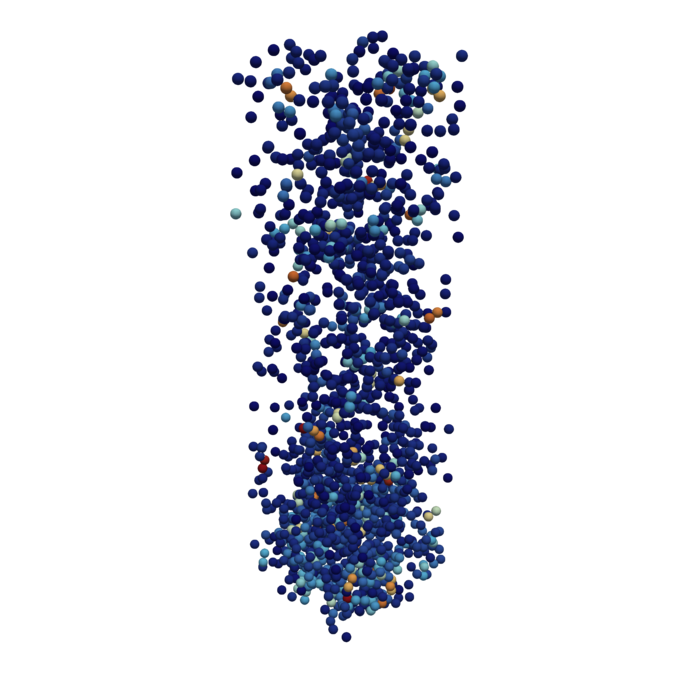
\includegraphics[width=\textwidth]{exploding-liquid/render/t51000.png}
		\subcaption{State at $t=51000$}
	\end{subfigure}%
	\hfill\begin{subfigure}[c]{.08\textwidth}
		\resizebox{\textwidth}{!}{
			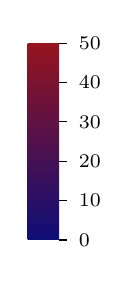
\begin{tikzpicture}
				\def\minval{0}
				\def\maxval{50}
				\definecolor{startcolor}{RGB}{14,14,120}
				\definecolor{midcolor}{RGB}{229,241,196}
				\definecolor{endcolor}{RGB}{150,20,30}
				\def\height{2.5}
				\def\width{0.4}
				\def\nsteps{5}
				
				\shade[top color=endcolor, color=midcolor, bottom color=startcolor] (0,0) rectangle (-\width,\height);
				
				\foreach \i in {0,...,\nsteps}{
					\pgfmathsetmacro{\val}{\minval + (\maxval-\minval)*\i/\nsteps}
					\pgfmathsetmacro{\y}{\height * (\val-\minval)/(\maxval-\minval)} 
					\draw (0.1,\y) -- (0,\y);
					\node[right, align=left] at (0.125,\y) {\scriptsize\pgfmathprintnumber[fixed,precision=2]{\val}};
				}
				% TODO: add unit for scale
			\end{tikzpicture}
		}
	\end{subfigure}
	\label{fig:evolution_expl}
	\caption{Evolution of the simulation state in the exploding liquid scenario.}
\end{figure}

\subsection{Heating Sphere}
\label{subsec:hs}
\begin{figure}[htpb]
	\centering
	\begin{subfigure}[c]{.3\textwidth}
		% \includegraphics[width=\textwidth]{heating-sphere/render/t0.png}
		\subcaption{State at $t=0$}
	\end{subfigure}%
	\begin{subfigure}[c]{.3\textwidth}
		% 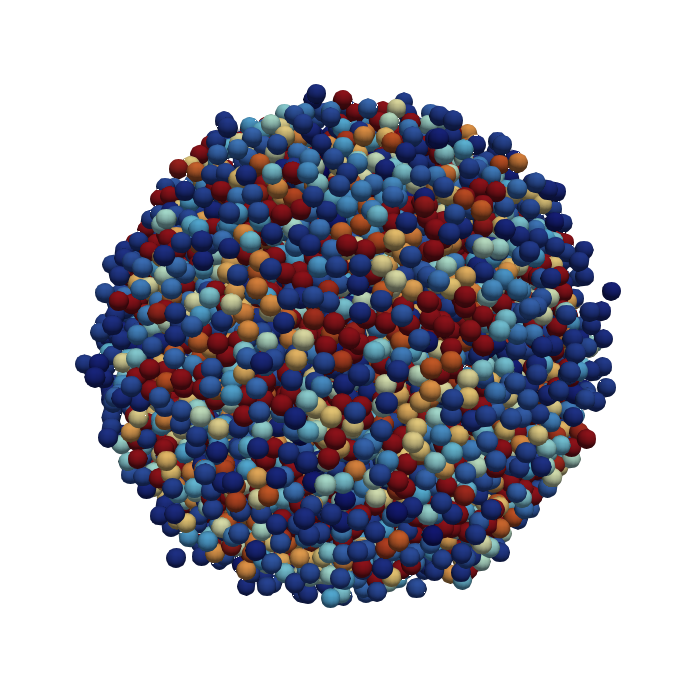
\includegraphics[width=\textwidth]{heating-sphere/render/t4000.png}
		\subcaption{State at $t=4000$}
	\end{subfigure}%
	\begin{subfigure}[c]{.3\textwidth}
		\centering
		% 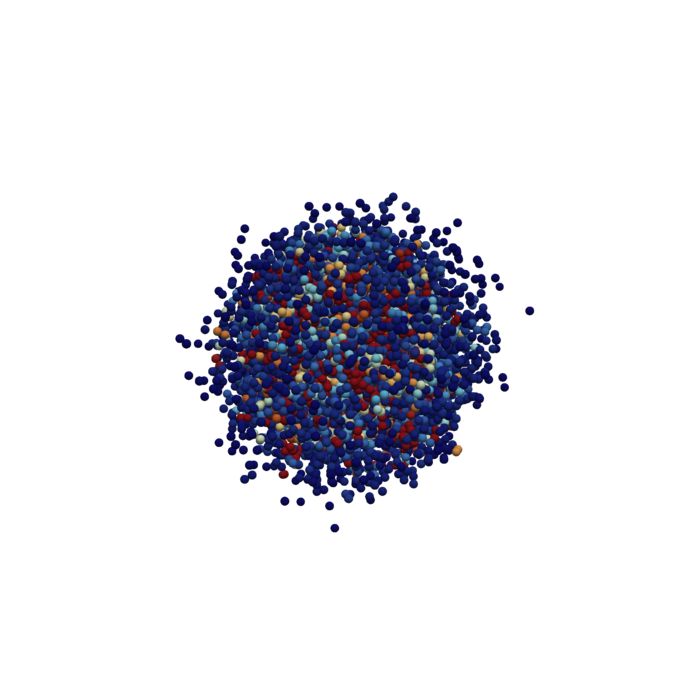
\includegraphics[width=\textwidth]{heating-sphere/render/t12000.png}
		\subcaption{State at $t=12000$}
	\end{subfigure}
	\hspace*{.15\textwidth}
	\begin{subfigure}[c]{.3\textwidth}
		% 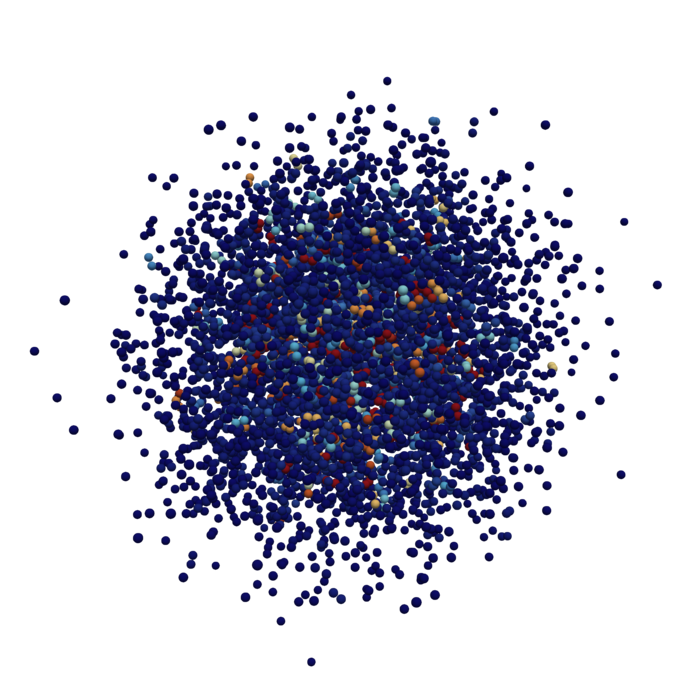
\includegraphics[width=\textwidth]{heating-sphere/render/t23000.png}
		\subcaption{State at $t=23000$}
	\end{subfigure}%
	\begin{subfigure}[c]{.3\textwidth}
		\vspace*{0.1\textwidth}
		\centering
		% 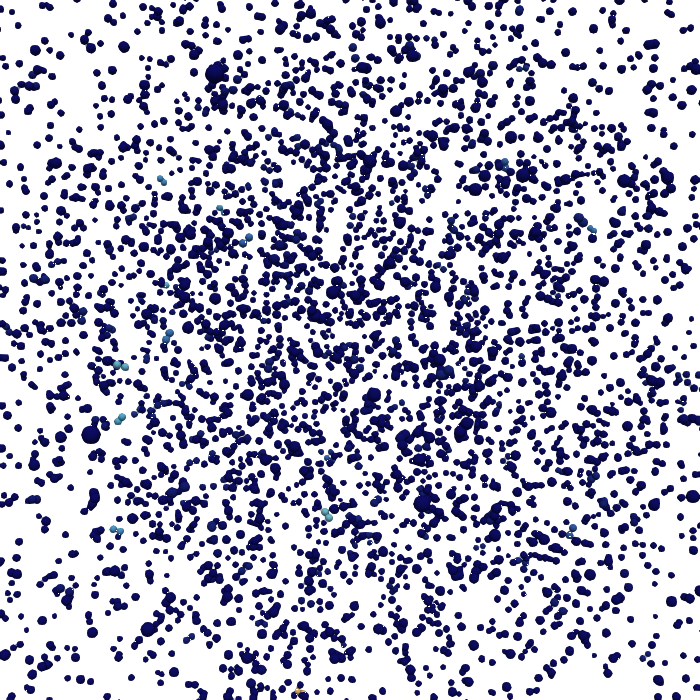
\includegraphics[width=0.8\textwidth]{heating-sphere/render/t60000.png}
		\vspace*{0.1\textwidth}
		\subcaption{State at $t=60000$}
	\end{subfigure}%
	\hfill\begin{subfigure}[c]{.08\textwidth}
		\resizebox{\textwidth}{!}{
			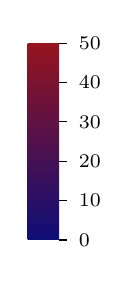
\begin{tikzpicture}
				\def\minval{0}
				\def\maxval{50}
				\definecolor{startcolor}{RGB}{14,14,120}
				\definecolor{midcolor}{RGB}{229,241,196}
				\definecolor{endcolor}{RGB}{150,20,30}
				\def\height{2.5}
				\def\width{0.4}
				\def\nsteps{5}
				
				\shade[top color=endcolor, color=midcolor, bottom color=startcolor] (0,0) rectangle (-\width,\height);
				
				\foreach \i in {0,...,\nsteps}{
					\pgfmathsetmacro{\val}{\minval + (\maxval-\minval)*\i/\nsteps}
					\pgfmathsetmacro{\y}{\height * (\val-\minval)/(\maxval-\minval)} 
					\draw (0.1,\y) -- (0,\y);
					\node[right, align=left] at (0.125,\y) {\scriptsize\pgfmathprintnumber[fixed,precision=2]{\val}};
				}
				% TODO: add unit for scale
			\end{tikzpicture}
		}
	\end{subfigure}
	\label{fig:evolution_hs}
	\caption{Evolution of the simulation state in the heating sphere scenario.}
\end{figure}

\subsection{Falling Drop}
\label{subsec:fd}
\subsection{Spinodial Decomposition}
\label{subsec:sd}

\section{Evaluation Metrics}
To compare results between dynamic and static tuning intervals, different metrics can be used. 
Firstly, the primary goal is to reduce the total simulation runtime for a range of typical scenarios. As tuning phases spend time without advancing the simulation result, a reduction in total runtime is the expected result if our approach reduces the number of tuning phases without spending too many iterations using a suboptimal configuration.

The metric of total runtime is not particularly fine-grained however, as it only takes into account entire simulation runs. To achieve a more detailed benchmark, we also consider the number of iterations that were running on an optimal configuration. As an approximation to the optimal configuration per iteration we use simulation run with static tuning, a high number of tuning samples and a short tuning interval. Based on this static data we can then rank the configuration our dynamic run chose in terms of \enquote{optimality}.

%Finally, the percentage of tuning iterations might be of interest. Depending on the tuning strategy used, the retuning process can terminate early. % TODO?
%Therefore, the actual number of iterations spent in a tuning phase might be different depending on the iteration in which that phase was started. In such cases, it might be beneficial to have more 


\section{Results}
\subsection{Optimality}
\subsection{Runtime}
\subsection{Share of tuning iterations}
\subsection{Trigger Parameters}
% sensible default values

